\chapter{System Model}
Cuttlefish, as mentioned earlier, is a 3D printing pipeline which performs the preprocessing of the 3D model and conversion of the virtual design to a form driving the print machine. The virtual blueprint of the object i.e. the digital model of the object to be printed is created using a designing software. Cuttlefish allows for numerous file formats like STL, Obj, Ply, Wrl as input giving the designer the flexibility to use a designing software of his choice. The whole pipeline has a streaming architecture, which means that the input can processed in smaller parts so as to generate the output sooner thus letting the printing process to be started as early as possible i.e. even before the whole object has been processed.The output is generated in parts called as \textit{chunks}- each chunk is a collection of 2D layers, where each layer is referred to as a \textit{slice}. \newline

\section{Non-distributed Cuttlefish Pipeline Components}

The pipeline along with streaming architecture has a component-based architecture as well. The composition of the pipeline varies as per the components assembled to form the pipeline. The components composing the pipeline can be chosen on the basis of factors like the type of generated output, for example \textit{Bitmaproducer} component is chosen as the output component if the desired output is bitmaps or \textit{STLProducerObjet} component is included when the desired output is STL file per print material i.e. a mesh representation or if the output required is a gcode (gcode is set of instructions to drive cnc machines) then the component used is GCodeProducer, and also some of the previously mentioned components can be included together as well to generate multiple types of output simultaneously in a single pipeline run. Another factor for deciding the components of the pipeline is the targeted printer machine i.e. if the targeted printing machine is single material or multi-material material printer. 
\newline

The pipeline performs the following fundamental steps in a serial fashion irrespective of the components forming the pipeline \ref{fig:TypicalCuttlefishSteps}. After the voxelization process, all the further processing happens in a chunk-wise manner. 

\begin{figure}[ht!]
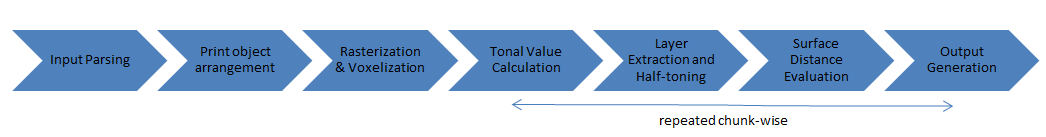
\includegraphics[scale=0.6]{TypicalCuttlefishSteps.PNG}
\caption{Cuttlefish pipeline component functionality}
\label{fig:TypicalCuttlefishSteps}
\end{figure}

\begin{itemize}
\item \textbf{Input Parsing}: The input given to the pipeline, mostly mesh files and textures, is parsed and internal mesh representations are created for them. Internal mesh representations of multiple objects can be grouped together with each having it\textquotesingle s own unique identifier and is known as a print job. At present FileParsePj is the component which performs this task. \newline 

\item \textbf{Print object arrangement}: The print jobs are arranged within the print volume to lower material consumption and print time.The arrangement of the print jobs is done by using a greedy approach where in the print jobs are sorted as per the extent of the bounding box of the print object and best-fit algorithm is applied on the sorted boxes so as to arrange the print objects as compactly as possible in the print volume. PrintJobOrganizer is currently handling this task. \newline 

\item \textbf{Rasterization and Voxelization}: Rasterization is the process of converting an image described in a vector graphics format(shapes) to raster images i.e. pixels or dots for output to the printer or storing it in bitmap format. In voxelization, the mesh representation is converted to voxel representation and each voxel intersecting the surface is assigned attributes like color, occupancy etc. Currently the component doing this is PrintJobVoxelizer. The algorithm used for voxelization can be varied using the component configuration and the description of the voxelization algorithms is beyond the scope of the thesis. \newline 
 
\item \textbf{Tonal Value Calculation}: This step involves calculation and assignment of tonal values from the optical features (RGB or BRDF data) of surface voxels. The tonal value computation is done with the help of a calculated ICC-profile  belonging to the specific printer. The component doing this is called TonalValueCalculator.

\item \textbf{Surface Distance Evaluation and Tonal Analyzer} (optional): The component evaluates the distance of voxels to the surface and assigns values of a given attribute (of the surface voxel)  to inner voxels within the specified mask distance.The Tonal value analyzer component reports summary statistics, comparing the half-toned signal to the original tonal values in easy to interpret graphs.\newline

\item \textbf{Layer Extraction and Half-toning}: It involves extraction of the layers below surface and storing them in a easily accessible way to be used later for half-toning. Half-toning is the process of creating half-tone image. An Half-tone image is comprised of discrete dots rather than continuous tones, when viewed from a distance, the dots blur together, creating the illusion of continuous lines and shapes which helps to save print material. \newline

\item \textbf{Output Generation}: The generated slices are then used to create the desired output i.e. bitmaps or STL files. The output files are then used to drive the print machine. \newline

\end{itemize} 

The input given to the printer driver is a main configuration file called as main\_conf.json and has json data describing various input fields. The main configuration file enlists the files describing the printer specification, component configuration, geometry, texture, logger type and output folder path. The printer specification file consists of the details related to the resolution of the printer, print volume, material names and unique identifier for each material, ICC profile etc. The component configuration enlists the components forming the pipeline and configuration parameters for each component. Listing \ref{lst:CC} is an example of the BitmapProducerObjet component configuration description. \newline

\begin{lstlisting}[language=json,label={lst:CC},caption={BitmapProducerObjet Component Configuration}]
{
	"type":"BitmapProducerObjet",
  "OutputPath": "Output/",
  "PrinterTextFileName": "printer_config.txt",
  "computeType":"multi-threaded",
  "pitchRequirement": "32",
	"unusedMaterial":"VeroClear"
}
\end{lstlisting}

The \textit{type} field denotes the name of the component and \textit{computeType} sets the component to run in a single-threaded or multi-threaded fashion. \textit{OutputPath} is used to set the path at which the component generates the bitmaps and \textit{pitchRequirement} value is used to make the bitmap width a multiple of the specified number. The component which parses the input main configuration file creates a \textit{printingSoftware} for the given component configuration. 

\section{System Model for Distributed Cuttlefish Pipeline}

The non-distributed cuttlefish pipeline runs on a single machine and therefore there is no particular machine specific action needed to be performed depending on the rank of the machine. For an application to run on a cluster of machines, sometimes it is necessary to perform additional steps which are specific to the rank of the node in the cluster. Before understanding the architecture of the distributed cuttlefish printer driver it is necessary to understand the architecture of the cluster, referred to as a distributed system, on which the driver is designed to run. 

\subsection{Introduction to distributed systems and its types}
Distributed system consists of autonomous systems (AS) connected through network which interact (if necessary) through message passing and most importantly give the user an illusion of being single large system \cite{DCE}. The main goal of distributed system is to connect the users and the available infrastructure i.e. IT resources in a transparent, open, cost-effective, reliable as well as scalable way. Transparency in distributed computing environment (DCE) means that the user is unaware of the underlying system complexities in terms of location of the AS, heterogeneity of the system hardware, concurrency and replication of the AS mainly to provide reliability and fault tolerance. Scalability refers to the property by which the number of AS in the DCE can be increased (scaled in) or decreased(scaled out) so as to provide best suited infrastructure to handle the fluctuating load (i.e. the amount of work to be done).The shared resources of the distributed system can be broadly classified as physical resources and virtual resources. The Figure\ref{fig:TypesOfResourceSharing} details the resources included in the two categorizes. 

\begin{figure}[ht!]
\centering
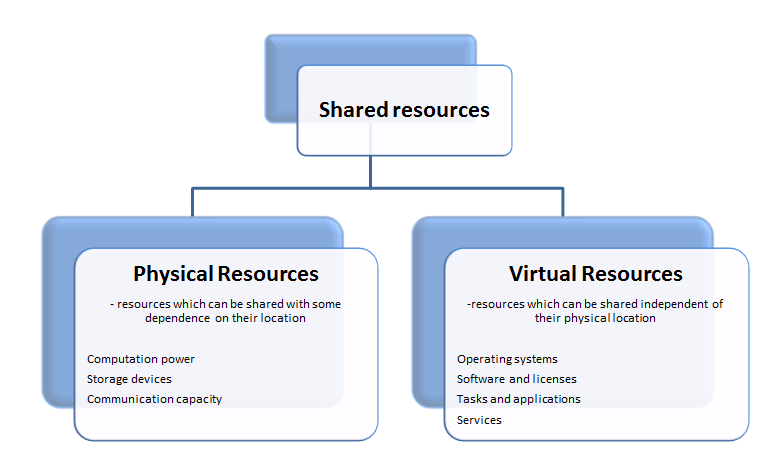
\includegraphics[scale=0.6]{TypesOfResourceSharing.PNG}
\caption{Distributed System Shared Resource Classification}
\label{fig:TypesOfResourceSharing}
\end{figure}
  
Distributed Computing is a vast domain which consists of various different types of computing environments like utility computing (grid computing and cloud computing), cluster computing, peer-to-peer computing and Jungle computing (figure \ref{fig:DistributedComputingEnv}). 

\begin{figure}[ht!]
\centering
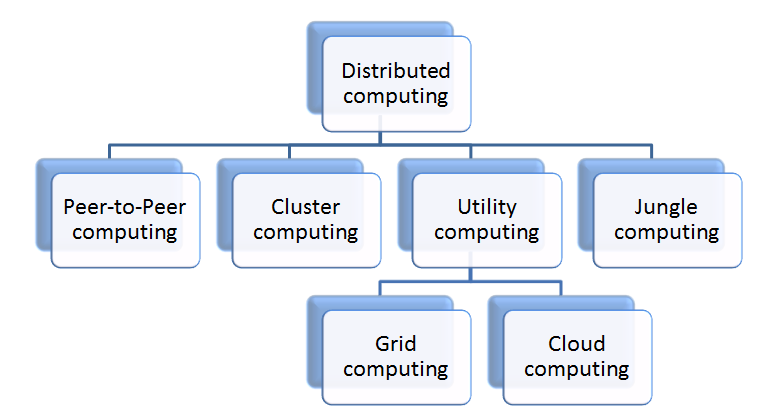
\includegraphics[scale=0.6]{DistributedComputingEnv.PNG}
\caption{Distributed Computing Environment}
\label{fig:DistributedComputingEnv}
\end{figure}

Each of the computing environment forming the part of the DCE is described briefly-
\begin{itemize}
\item \textbf{Peer-to-Peer computing}- Each node in the DCE acts as both client and server, providing as well as consuming part of the system resources. Peers are machines simply connected to the internet where in each peer can freely join and leave the DCE without affecting the whole system, implying no particular role(either master or slave) for a peer, making such a system self-organizing (figure \ref{fig:P2P}).

\begin{figure}[ht!]
\centering
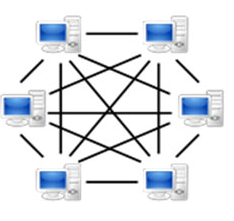
\includegraphics[scale=0.6]{P2P.PNG}
\caption{Peer-to-Peer system}
\label{fig:P2P}
\end{figure}

\item \textbf{Utility computing}- Utility computing is based on a model for service provisioning, which allows the users (consumers) to pay the providers for using the service only when they need to. It emphasizes on a business model, by which services provide make available the requested/paid resources to the costumers. All grid/cloud platforms are regarded as utility service providers. Grid computing is to enable coordinated resource sharing and problem solving in dynamic, multi-institutional virtual organizations where as cloud computing is a computing paradigm that involves outsourcing of computing resources with the capabilities of expendable resource scalability, on-demand provisioning with little or no up-front IT infrastructure investment costs. Cloud computing offers its benefits through
three types of service or delivery models namely infrastructure-as-a-service (IaaS), platform-as-a-service(PaaS) and software-as-a-Service (SaaS) 

\item \textbf{Cluster Computing}- A cluster comprises a set of independent or stand-alone computers and a network interconnecting them. It
works cooperatively together as a single integrated computing resource. A cluster is local in that all of its component subsystems are supervised within a single administrative domain, usually residing in a single room and managed as a single computer system. The components of a cluster are connected to each other through fast local area networks. 

\item \textbf{Jungle Computing}- It is the combination of one or more DCEs enlisted above resulting in a highly diverse, distributed and non-uniform high performance computing environments (figure \ref{fig:JungleComputing}).  

\begin{figure}[ht!]
\centering
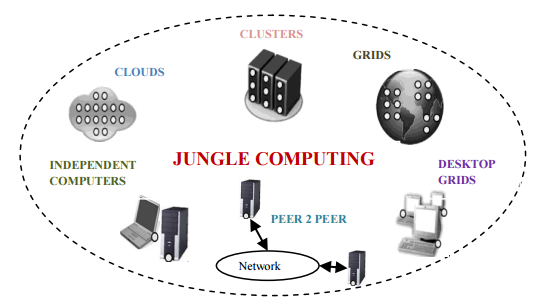
\includegraphics[scale=0.6]{JungleComputing.PNG}
\caption{Jungle Computing}
\label{fig:JungleComputing}
\end{figure}

\end{itemize}

\subsection{Distributed system for cuttlefish printer driver}

The distributed cuttlefish printer driver is developed using a cluster of the computers(nodes) which are heterogeneous in their hardware as well as software configuration and are connected via the Fraunhofer network. The initial set up used during the development had three nodes out of which one node is the master node and remaining nodes are the slave nodes. The names master and slave depict a predetermined role the nodes have and type of work they do. The nodes also have access to a shared networked file system (figure \ref{fig:CuttlefishCluster}).

\begin{figure}[ht!]
\centering
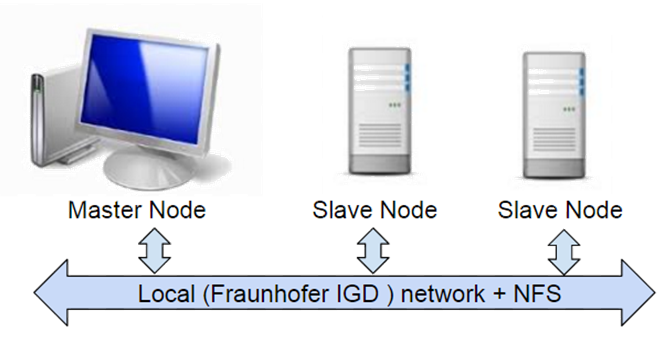
\includegraphics[scale=0.6]{CuttlefishCluster.PNG}
\caption{Cluster setup}
\label{fig:CuttlefishCluster}
\end{figure}

As mentioned earlier, the role of the node determines the type of work they do.The master node is the computer in the cluster where the user submits his request, namely the main configuration file (figure \ref{fig:Step1}). 

\begin{figure}[ht!]
\centering
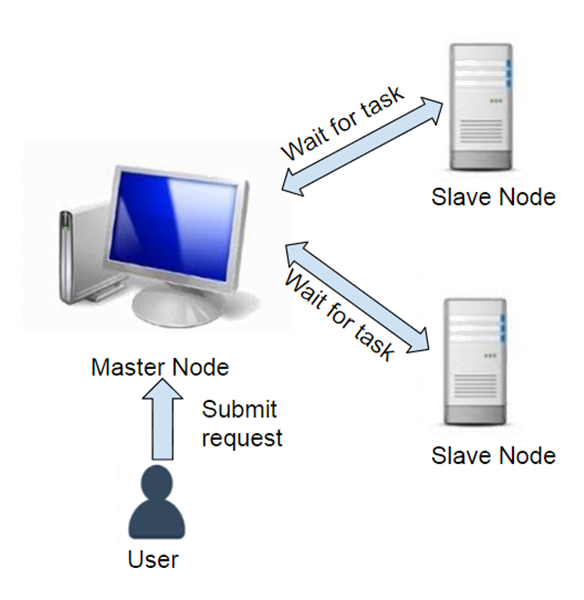
\includegraphics[scale=0.6]{Step1.PNG}
\caption{User submits the request}
\label{fig:Step1}
\end{figure}

The master node then performs some computation and distributes the sub-tasks to be performed by the slave nodes (figure \ref{fig:Step2}). 

\begin{figure}[ht!]
\centering
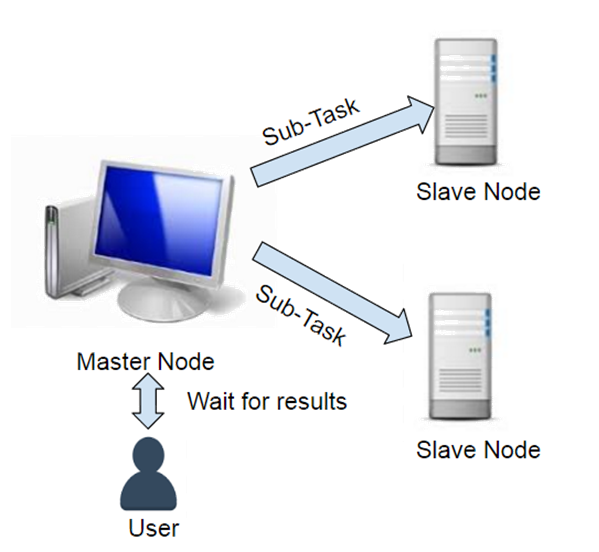
\includegraphics[scale=0.6]{Step2.PNG}
\caption{Master distributes the sub-tasks}
\label{fig:Step2}
\end{figure}

The slave nodes perform the assigned tasks and report back to the master (figure \ref{fig:Step3}). The cluster nodes follow a classic \textit{master-slave} communication paradigm. 

\begin{figure}[ht!]
\centering
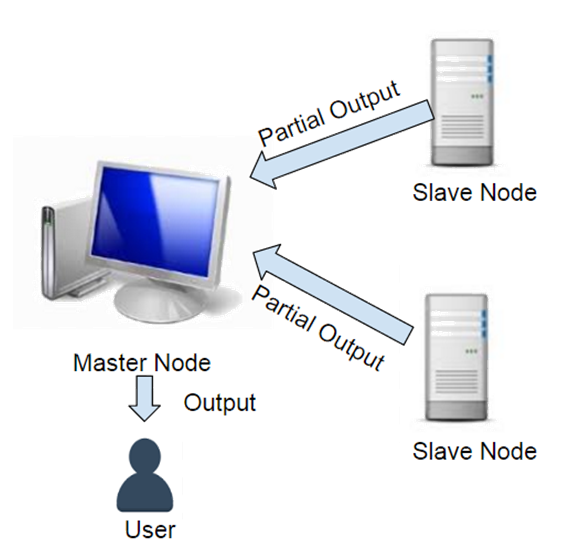
\includegraphics[scale=0.6]{Step3.PNG}
\caption{Slaves report the partial output}
\label{fig:Step3}
\end{figure}

\subsection{Components of distributed cuttlefish printer driver}

The distributed cuttlefish pipeline components may differ depending upon the role of the node in the cluster. The components put together form a printing software in which the components run on the node in a loop, with each iteration of the loop processing chunk-wise data. To apply distributed computing as a solution for stated problem of large computation on big data set, there are three additional steps, as enlisted below, some of which need to be performed either on the master or the slave node:  
\begin{enumerate}
\item Division of task into sub-tasks 
\item Awaiting the sub-tasks and doing the needed work
\item Submitting back the partial output
\end{enumerate}

\subsubsection{Master Node Printing Software Components}
As per the model discussed in the earlier section, the master node performs the step $1$ from the above enlisted steps. The division of the task among the slave nodes needs to be performed by the master efficiently so as to make sure that distributed load is balanced and none of the slaves are over-worked. To do so, the master needs to evaluate the input and perform some measurements so as to make a wise decision regarding the task split. Hence, the master printing software needs to at least parse the input into an internal mesh representation i.e.\textit{printjobs} and compute the necessary parameters on the basis of which an informed decision can be made. The component \textit{MasterDistributor} is responsible for division of the submitted task and takes the \textit{printjobs} as input and generates sub-tasks as the output. After the successful generation of the sub-tasks, the distribution of the sub-tasks among the slaves is done. The form in which the tasks are distributed may vary leading to different designs of the component which is discussed in detail in the next chapter. 

On receiving the sub-tasks from the master, the slave nodes start doing their share of work. The master after submitting the sub-tasks has to wait for the slaves to generate the partial output. So as to maintain the streaming architecture, the slaves perform the assigned work in parts and report the partial output to the master. The master then collects the partial output and performs some computation using received data and provides the final output to the user. \textit{MasterMerger} component in the master printing pipeline is responsible for receiving the partial output and later providing the final output to the user. The output from the slave nodes are the chunks of partial \textit{slices} which are later merged into final output i.e. chunks of full slices. Figure \ref{fig:MasterPS} shows the components of the printing software running on the master node.
\begin{figure}[ht!]
\centering
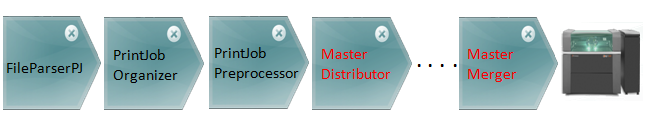
\includegraphics[scale=0.8]{MasterPS.PNG}
\caption{Master Node Printing Software Components }
\label{fig:MasterPS}
\end{figure}


\subsubsection{Slave Node Printing Software Components}

The slave nodes in the cluster (i.e. all nodes other than the master are considered slave nodes) perform the assigned task and report back the results to the master node. To do so, the slaves nodes have to first wait until the master has divided the task submitted by the user into smaller sub-tasks. Once receiving the input, the slave nodes run the whole printing software (similar to the non-distributed cuttlefish version) with just one minor change. As the slave nodes report the partial output to the master, they do not need to run the output component, for example the bitmapproducer. The partial output which is reported by the slaves to master is in form of \textit{slices} and hence, the slave printing software running on the slave nodes does not contain the output component, instead it runs a component called the \textit{SlaveReporter} which, as the name suggests, reports the partial output in a chunk-wise fashion back to the master. Figure \ref{fig:SlavePS} shows the components of the printing software running on the slave node.
\begin{figure}[ht!]
\centering
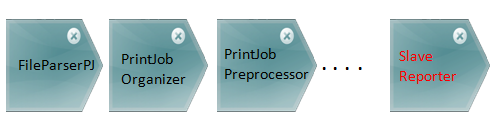
\includegraphics[scale=0.8]{SlavePS.PNG}
\caption{Slave Node Printing Software Components }
\label{fig:SlavePS}
\end{figure}

